\documentclass[12pt]{article}
\usepackage{geometry}                % See geometry.pdf to learn the layout options. There are lots.
\geometry{letterpaper}                   % ... or a4paper or a5paper or ... 
%\geometry{landscape}                % Activate for for rotated page geometry
\usepackage[parfill]{parskip}    % Activate to begin paragraphs with an empty line rather than an indent
\usepackage{daves,fancyhdr,natbib,graphicx,dcolumn,amsmath,lastpage,url}
\usepackage{amsmath,amssymb,epstopdf,longtable}
\usepackage{paralist}  % need to properly formulate standard answer blocks
\DeclareGraphicsRule{.tif}{png}{.png}{`convert #1 `dirname #1`/`basename #1 .tif`.png}
\pagestyle{fancy}
\lhead{CE 3372 Water Systems Design; Exam 1}
\rhead{\textbf{Name \_\_\_\_\_\_\_\_\_\_\_\_\_\_\_\_\_\_\_\_\_\_\_\_\_\_\_\_\_\_\_\_\_\_}}
\lfoot{REVISION A}
\cfoot{}
\rfoot{Page \thepage\ of \pageref{LastPage}}
\renewcommand\headrulewidth{0pt}



\begin{document}
\begingroup
\begin{center}
{\textbf{{ CE 3372 Water Systems Design} \\ Exam 1 \\ Spring 2025} }
%{\textbf{{ CE 3372 Water Systems Design} \\ Quiz 1 \\ Fall 2014} }
\end{center}
\endgroup


\begin{enumerate}
%%%%%%%%%%%%%%%%%%%%%%%%%%%%%%%%%%%%%
\item What is a water use system? How are they usually sized?\\
\item What is a water control system? How are they usually sized?\\
\item Which kind of system is depicted in Figure \ref{fig:whiteoakbayou}?  Explain your reasoning.
\begin{figure}[h!] %  figure placement: here, top, bottom, or page
   \centering
   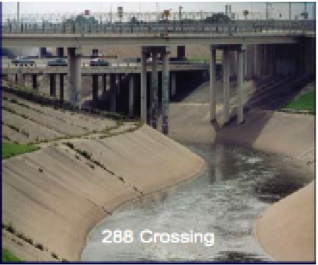
\includegraphics[width=4in]{whiteoakbayou.jpg} 
   \caption{Braes Bayou at SH288}
   \label{fig:whiteoakbayou}
\end{figure}

\item Use Title 30, Part 1, Chapter 290, Subchapter D, Rule 290.44 of the Texas Administrative Code or TCEQ RG-195 to find the minimum pressure requirement for a public water system during normal (non-fire suppression) operation for parts of the system that deliver 1.5 gallons per minute or more.\\
\clearpage
\item Use Title 30, Part 1, Chapter 290, Subchapter D, Rule 290.44 of the Texas Administrative Code or TCEQ RG-195 to find the minimum pressure requirement for a public water system during emergency (fire suppression) operation for parts of the system that deliver 1.5 gallons per minute or more.\\
\item Use Title 30, Part 1, Chapter 290, Subchapter D, Rule 290.44 of the Texas Administrative Code or TCEQ RG-195 to find the minimum distance (spacing) for new potable water distribution lines in feet to wastewater collection facilities.\\
\item Use Title 30, Part 1, Chapter 290, Subchapter D, Rule 290.44 of the Texas Administrative Code or TCEQ RG-195 to find the minimum free chlorine residual in mg/L required in Texas water distribution systems (if using free chlorine).\\
\item Consider the two networks depicted in the Figure below. Both network designs serve the same junction nodes, have same nodal demands, and draw supply from the same reservoir.

\begin{figure}[h!] %  figure placement: here, top, bottom, or page
   \centering
   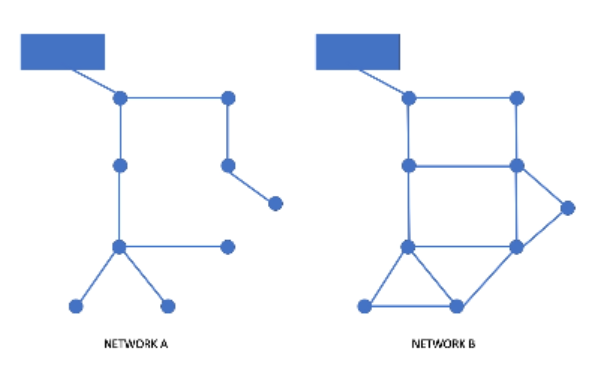
\includegraphics[width=4in]{Distribution.png} 
   \caption{Two Distribution Systems}
   \label{fig:placeholder0}
\end{figure}

Which network design would be superior in terms of reliability? Why? \\

\clearpage

\item Consider the two networks depicted in the Figure below. Both network designs serve the same junction nodes, have same nodal demands, and draw supply from the same reservoir.

\begin{figure}[htbp] %  figure placement: here, top, bottom, or page
   \centering
   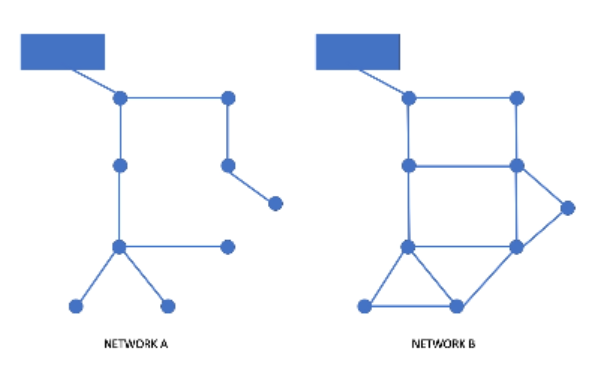
\includegraphics[width=4in]{Distribution.png} 
   \caption{Two Distribution Systems}
   \label{fig:placeholder1}
\end{figure}

Which network design would cost less to build? Why?  \\

\item Consider the two networks depicted in the Figure below. Both network designs serve the same junction nodes, have same nodal demands, and draw supply from the same reservoir.

\begin{figure}[htbp] %  figure placement: here, top, bottom, or page
   \centering
   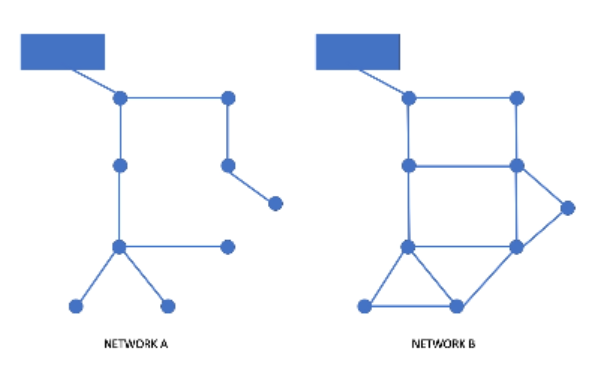
\includegraphics[width=4in]{Distribution.png} 
   \caption{Two Distribution Systems}
   \label{fig:placeholder2}
\end{figure}

Which network would be superior in terms of disinfection residual? Why? \\

\item Consider the pipe network portion shown in the Figure below. Node 6 has a total head of 290.5 meters. All the pipes are PVC (roughness height = 0.007 millimeters).  What is the discharge in cubic meters per second (cms) in pipe P1?

\begin{figure}[h!] %  figure placement: here, top, bottom, or page
   \centering
   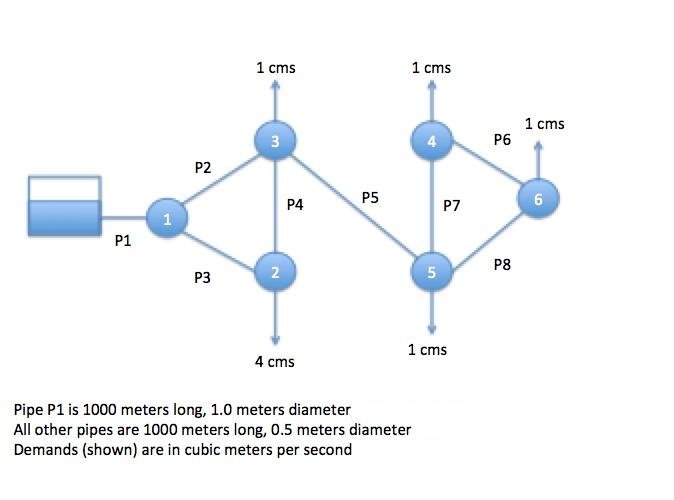
\includegraphics[width=3.5in]{2018Pipeline2.jpg} 
   \caption{A Distribution System}
   \label{fig:placeholder3}
\end{figure}

\item Consider the pipe network portion shown in the Figure below. Node 6 has a total head of 290.5 meters. All the pipes are PVC (roughness height = 0.007 millimeters).  What is the discharge in cubic meters per second (cms) in pipe P5?

\begin{figure}[h!] %  figure placement: here, top, bottom, or page
   \centering
   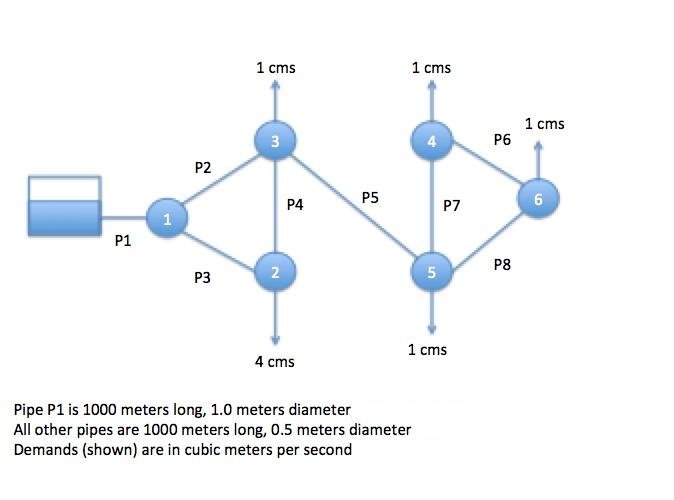
\includegraphics[width=3.5in]{2018Pipeline2.jpg} 
   \caption{A Distribution System}
   \label{fig:placeholder4}
\end{figure}
\clearpage

\item Consider the pipe network portion shown in the Figure below. Node 6 has a total head of 290.5 meters. All the pipes are PVC (roughness height = 0.007 millimeters).  What is the discharge in cubic meters per second (cms) in pipe P6?

\begin{figure}[htbp] %  figure placement: here, top, bottom, or page
   \centering
  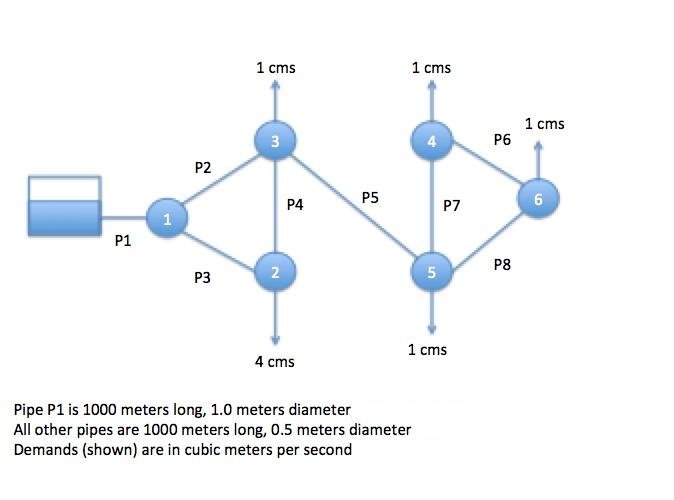
\includegraphics[width=3.5in]{2018Pipeline2.jpg} 
   \caption{A Distribution System}
   \label{fig:placeholder5}
\end{figure}

\item The pressure drop across a valve, through which 0.04 cubic meters per second of water flows, is measured to be 100 kPa. Estimate the loss coefficient if the nominal diameter of the valve is 8 cm. \\

\clearpage

\item The figure below is a perspective view of a large at-grade water storage reservoir. The initial depth in the 50-foot diameter tank is  Z = 30 feet. What is the average outflow rate in cubic-feet-per-second, if the tank drains through the hole in the side in 24 hours? 

\begin{figure}[htbp] %  figure placement: here, top, bottom, or page
   \centering
  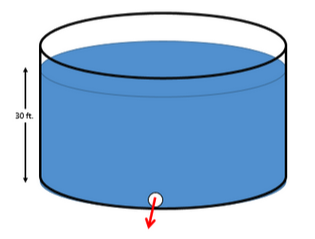
\includegraphics[width=4in]{StorageTank.png} 
   \caption{At-grade storage reservoir}
   \label{fig:placeholder6}
\end{figure}

\item Figure \ref{fig:PumpPlantPicture} is a collection of annotated images of the Edmonston Pumping Plant and pipeline/tunnel system at the southern end of the California Aqueduct.  The 10+ mile system lifts water from the Edmonston forebay at elevation 1239 feet to the Tehachapi afterbay at elevation 3131 feet for subsequent distribution to various parts of southern California.

Figure %\ref{fig:pumpcurve} 
is a pump performance curve for one of the 14 pumps arranged in two 7-pump bays, each supplying one of the parallel 16-foot diameter steel pressure pipes. 
\begin{figure}[ht!] %  figure placement: here, top, bottom, or page
   \centering
   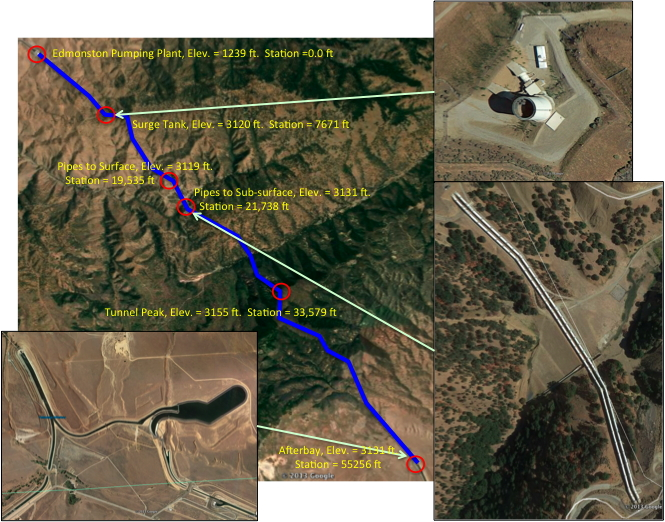
\includegraphics[width=6.5in]{PumpPlantPicture.jpg} 
   \caption{Aerial images of Tehachapi Mountains, California;  showing the lift system for the California Aqueduct.}
   \label{fig:PumpPlantPicture}
\end{figure}

\begin{figure}[ht!] %  figure placement: here, top, bottom, or page
   \centering
   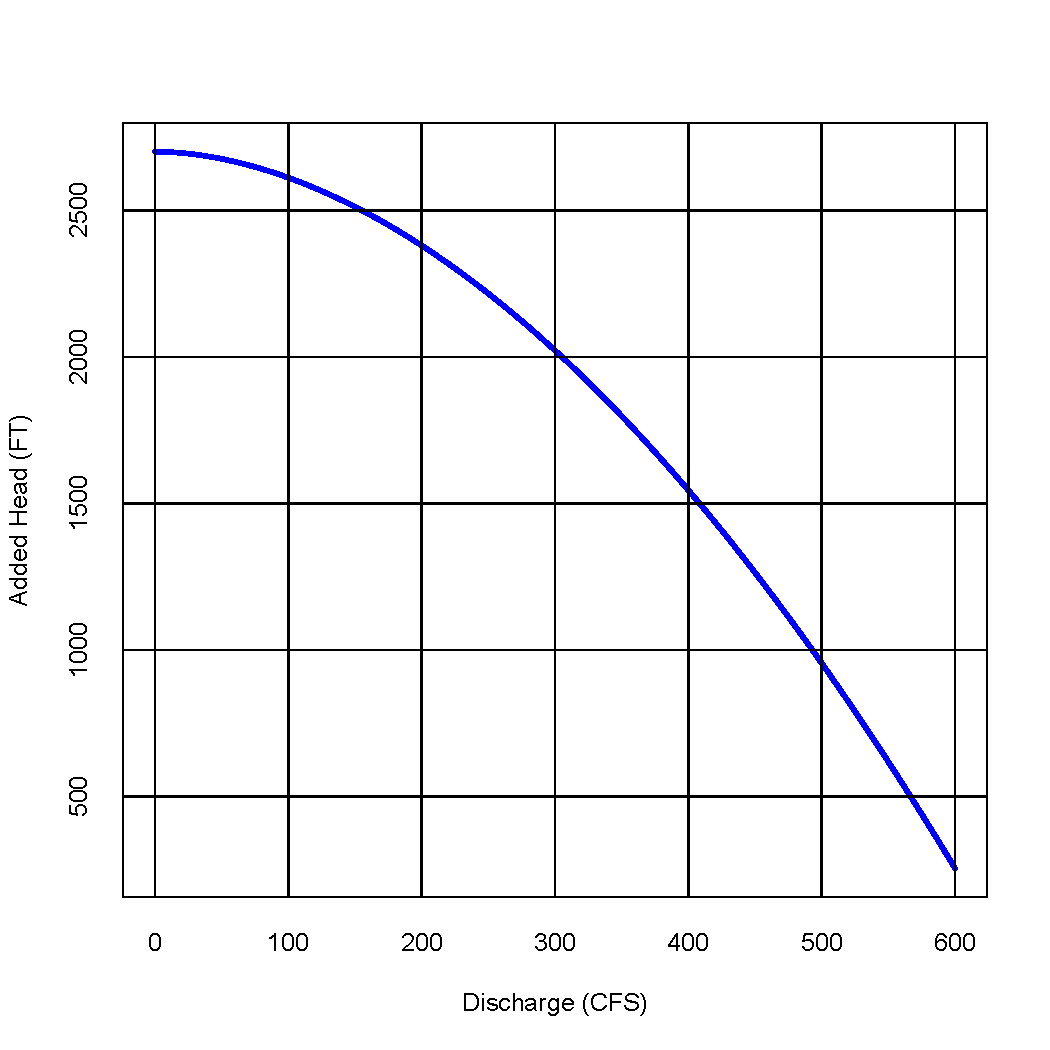
\includegraphics[width=6in]{pumpcurve.pdf} 
   \caption{Lift pump performance curve for single pump.   System has 14 identical pumps in two parallel galleries;  each gallery has 7 pumps operating in parallel.}
   \label{fig:pumpcurve}
\end{figure}

    \begin{enumerate}[a)]
    %%%%%%%%%%%%%%%%%%%%%%%%
\item Sketch a plan view layout of the system showing the various components, and station distances (from the pump station forebay).  Label the sketch with node elevations, node names, pipe names, and pipe lengths.).
\item What are the pipe lengths between the indicated locations in Table \ref{tab:lengths} (i.e. complete the table)?
\begin{table}[h!]
   \centering
    \caption{Selected Pipeline Locations and Pressures }
   \begin{tabular}{p{0.5in}p{1.8in}p{1in}p{1in}p{1in}} % Column formatting, @{} suppresses leading/trailing space
\hline
\hline
ID & Location & Distance from Pumps (feet) & Connection Sequence & Pipe Barrel Length  \\
\hline
\hline
1& Edmonston Pump House & ~~~~~0  & N/A & 0 \\
\hline
2& Surge Tank & ~7,671 & 1 to 2 & ~~ \\
\hline
3& Pipes to Surface & 19,535 & 2 to 3 & ~~ \\
\hline
4& Pipes to Ground & 21,738 & 3 to 4 & ~~ \\
\hline
5& High Tunnel & 33,579 & 4 to 5 & ~~ \\
\hline
6& Tehachapi Afterbay & 55,256 & 5 to 6 & ~~ \\
\hline
   \end{tabular}
   \label{tab:lengths}
\end{table}
\item What is the total length of pipe/tunnel required (in miles)?
\item What is the total head at the Edmonston Pump Forebay (the pumphouse)?
\item What hydraulic element is used to represent the forebay?
\item What is the total head at the Tehachapi Afterbay?
\item What hydraulic element is used to represent the afterbay?
\item What head-loss model is most appropriate for this analysis?
\item What is the total discharge in the system in cubic-feet-per-second when all 14 pumps are running?
\item What is the pressure at the locations in Table \ref{tab:pressures} (i.e. complete the table)?
\begin{table}[h!]
   \centering
    \caption{Selected Pipeline Locations and Pressures }
   \begin{tabular}{p{0.5in}p{2in}p{1in}p{0.7in}p{0.7in}} % Column formatting, @{} suppresses leading/trailing space
\hline
\hline
ID & Location & Distance from Pumps (feet) & Elevation (feet) & Pressure (psi) \\
\hline
\hline
0& Edmonston Pump House (suction) & ~~~~~0  & 1,239 & ~~ \\
\hline
0& Edmonston Pump House (discharge)& ~~~~~0  & 1,239 & ~~ \\
\hline
2& Surge Tank & ~7,671 & 3,121 & ~~ \\
\hline
3& Pipes to Surface & 19,535 & 3,119 & ~~ \\
\hline
4& Pipes to Ground & 21,738 & 3,131 & ~~ \\
\hline
5& High Tunnel & 33,579 & 3,566 & ~~ \\
\hline
6& Tehachapi Afterbay & 55,256 & 3,131 & ~~ \\
\hline
   \end{tabular}
   \label{tab:pressures}
\end{table}
\item What is the velocity of water the each of the pipes?
\item What is the mechanical energy required to move the water in kW-h  (kilowatt-hours)?
    %%%%%%%%%%%%%%%%%%%%%
    \end{enumerate}
%%%%%%%%%%%%%%%%%%%%%
\end{enumerate}
\end{document}  